\subsection{Formuláře}
Jednou z komplikovanějších částí implementace bylo vytvoření formulářů pro přidávání a úpravu událostí. Symfony poskytuje propracovaný systém pro práci s formuláři, který zahrnuje jejich vytváření, renderování, zpracování nebo i validaci. Součástí zpracování formuláře je i možnost jeho propojení s konkrétním objektem, díky čemuž se vyplněné hodnoty do tohoto objektu automaticky propisují. Validace vyplněných hodnot probíhá jak na straně klienta díky speciálním atributům u tagu \mintinline{text}|input|, tak na straně serveru, kde je řešena s využitím Symfony validátorů, konkrétně pomocí „Symfony Validation Constraints“.

Pro vlastnosti objektu \mintinline{text}|Event|, jež jsou typu \mintinline{text}|string|, \mintinline{text}|integer| nebo \mintinline{text}|datetime|, nebylo vytváření formuláře nijak speciální. Zajímavější bylo vymyslet, jakým způsobem do formuláře přidat vlastnosti \mintinline{text}|categories| a \mintinline{text}|organizers|, která jsou v databázi reprezentované vazbou M:N mezi entitami \mintinline{text}|Event| a \mintinline{text}|Category|, respektive \mintinline{text}|Event| a \mintinline{text}|Organizer|. Uvedený typ vazby M:N v případě entit \mintinline{text}|Event| a \mintinline{text}|Category| znamená, že událost může mít libovolné množství kategorií a naopak konkrétní kategorie může být přiřazena k libovolnému počtu událostí.

Po zvážení dostupných možností jsem se rozhodl vytvořit formulář, ve kterém je možné dynamicky přidávat a odebírat nové kategorie a organizátory. Nové položky lze do formuláře přidat vybráním již existujícího záznamu registrovaného u jiné události, nebo vytvořením zcela nové položky. Finální vzhled části formuláře obsahující sekci s kategoriemi je zobrazen na obrázku \ref{figure:form}.

\begin{figure}[h]
    \caption{Část formuláře na přidání události}
    \label{figure:form}
    \centering
    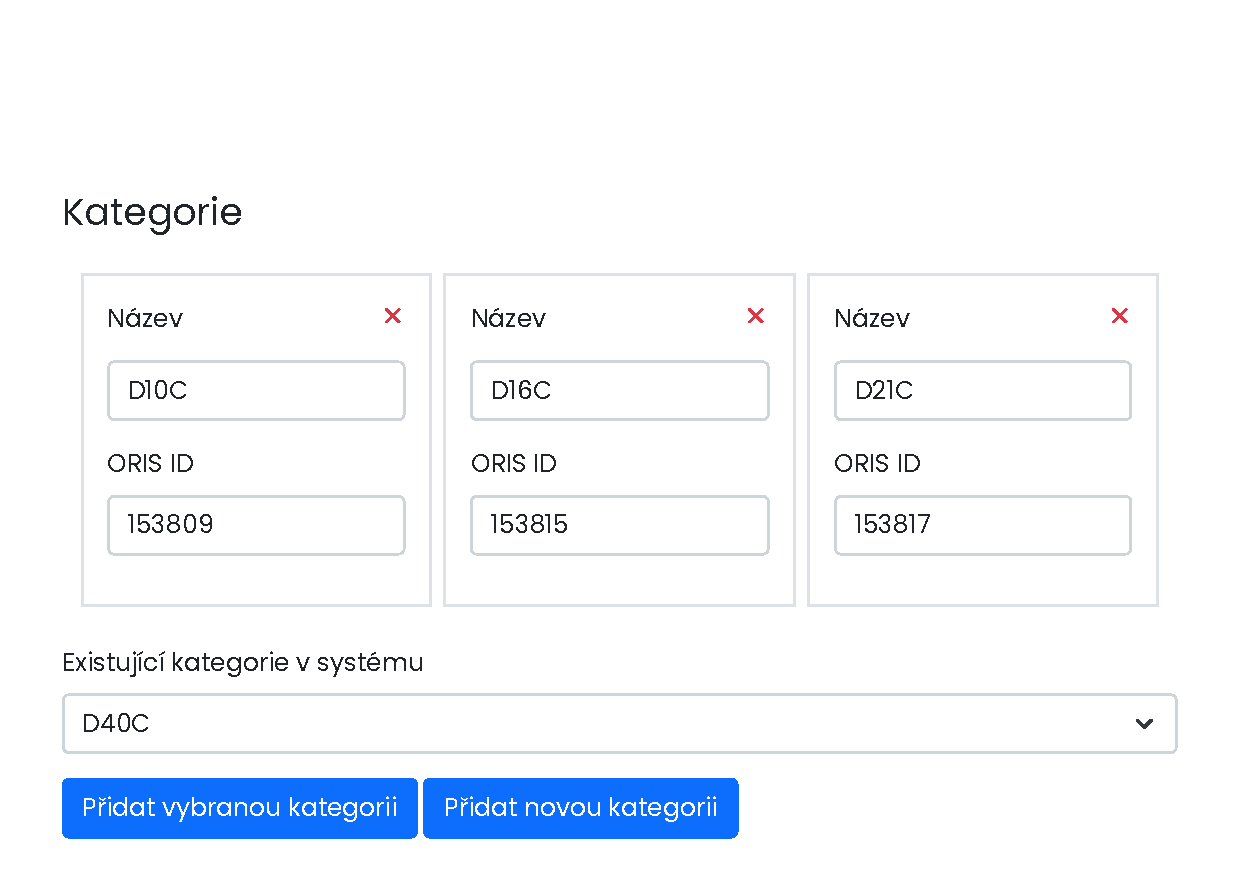
\includegraphics[width=0.947\linewidth, cfbox=kuorisgray 0.5pt 10pt]{images/form.pdf}
\end{figure}

Logiku ukládání a odebírání položek nebylo třeba vymýšlet od začátku, poněvadž Symfony formuláře obsahují podporu pro přidávání libovolného počtu položek ke kontrétní vlastnosti. Pro~zprovoznění této funkcionality však bylo nezbytné přidat vlastní kód v jazyku JavaScript, který zařídí samotné přidávání a odebírání položek z objektového modelu dokumentu (DOM). V souvislosti s dynamickým přidáváním nových položek bylo nutné navíc zamezit jejich duplikování v databázi v případě shody hodnot jejich vlastností.
